% Use Roman numerals (i, ii, iii, etc.) for page numbers in the front matter.
\pagenumbering{roman}

%%%%%%%%%%%%%%%%%%%%%%%%%%%%%%%%%%%%%%%%%%%%%%%%%%%%%%%%%%%%%%%%%
%% TITLE PAGE.
%%%%%%%%%%%%%%%%%%%%%%%%%%%%%%%%%%%%%%%%%%%%%%%%%%%%%%%%%%%%%%%%%

% No headers or footers on the title page.
\thispagestyle{empty}

\begingroup
\centering
\setstretch{1.0}
~
\\[1em]
\sffamily\bfseries\fontsize{26}{31.2}\selectfont
\DocumentTitle
\\
Use Manual Line Breaks If Necessary
\\[0.4in]
\normalfont\large
Thesis by
\\[0.25em]
\sffamily\bfseries\Large
\AuthorName
\\[0.4in]
\normalfont\normalsize
In Partial Fulfillment of the Requirements
\\[0.5em]
for the Degree of
\\[0.5em]
Doctor of Philosophy
\\[0.5em]
in
\\[0.5em]
Electrical Engineering and Computer Science
\vfill
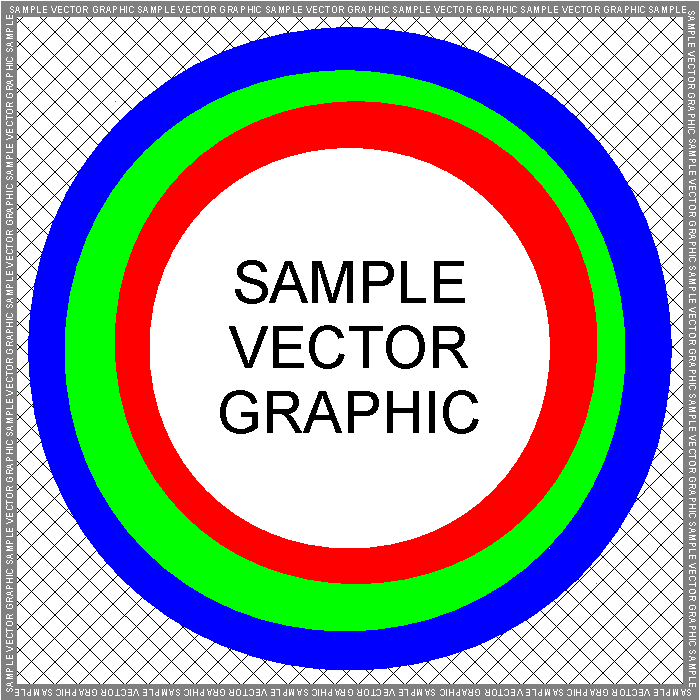
\includegraphics[height=1.8in]
{./Figures/Figure-SampleVectorGraphic}
\\[1.5em]
University Institute of College
\\[0.5em]
Springfield, New York, USA
\\[1.5em]
2016
\\[0.5em]
(Defended November 25, 2016)
\par
\endgroup

\clearpage

%%%%%%%%%%%%%%%%%%%%%%%%%%%%%%%%%%%%%%%%%%%%%%%%%%%%%%%%%%%%%%%%%
%% COPYRIGHT PAGE.
%%%%%%%%%%%%%%%%%%%%%%%%%%%%%%%%%%%%%%%%%%%%%%%%%%%%%%%%%%%%%%%%%

\pagestyle{plain}
\setcounter{page}{2}

\begingroup
\centering
\setstretch{1.0}
\null
\vfill
{\sffamily\textcopyright}~2016
\\[0.5em]
\AuthorName
\\[0.5em]
All Rights Reserved
\par
\endgroup

\clearpage

%%%%%%%%%%%%%%%%%%%%%%%%%%%%%%%%%%%%%%%%%%%%%%%%%%%%%%%%%%%%%%%%%
%% DEDICATION PAGE.
%%%%%%%%%%%%%%%%%%%%%%%%%%%%%%%%%%%%%%%%%%%%%%%%%%%%%%%%%%%%%%%%%

\begingroup
\centering
\setstretch{1.0}
~
\\[1in]
\textit{Insert dedication here}
\par
\endgroup

\clearpage

%%%%%%%%%%%%%%%%%%%%%%%%%%%%%%%%%%%%%%%%%%%%%%%%%%%%%%%%%%%%%%%%%
%% ACKNOWLEDGMENTS.
%%%%%%%%%%%%%%%%%%%%%%%%%%%%%%%%%%%%%%%%%%%%%%%%%%%%%%%%%%%%%%%%%

\chapter*{Acknowledgments}
\addcontentsline{toc}{chapter}{Acknowledgments}

{\color{red}%
Insert thesis acknowledgments here.
Thesis acknowledgments typically include research advisers and mentors, thesis committee members, collaborators, and funding sources.}

\lipsum[1-2]

\clearpage

%%%%%%%%%%%%%%%%%%%%%%%%%%%%%%%%%%%%%%%%%%%%%%%%%%%%%%%%%%%%%%%%%
%% ABSTRACT.
%%%%%%%%%%%%%%%%%%%%%%%%%%%%%%%%%%%%%%%%%%%%%%%%%%%%%%%%%%%%%%%%%

\chapter*{Abstract}
\addcontentsline{toc}{chapter}{Abstract}

{\color{red}%
Insert thesis abstract here.
The thesis abstract provides a concise description of the main contributions in the thesis.
Abstracting and indexing services usually include the thesis abstract in the catalog presented to users.
A well-written abstract could improve the chances of your work being discovered and cited by others in the research community.
The abstract should be self-contained (avoid citations and cross references) and should contain only plain text (avoid complicated mathematical expressions).}

\lipsum[1-6]

\clearpage

%%%%%%%%%%%%%%%%%%%%%%%%%%%%%%%%%%%%%%%%%%%%%%%%%%%%%%%%%%%%%%%%%
%% TABLE OF CONTENTS (TOC), LISTS OF FIGURES, TABLES, ETC.
%%%%%%%%%%%%%%%%%%%%%%%%%%%%%%%%%%%%%%%%%%%%%%%%%%%%%%%%%%%%%%%%%

\tableofcontents

\listoffigures

\listoftables

\clearpage

% Use Arabic numerals (1, 2, 3, etc.) for subsequent page numbers.
\pagenumbering{arabic}
